\documentclass[11pt]{article}
\usepackage[margin=0.8in]{geometry}
\usepackage[T1]{fontenc}
\usepackage{lmodern}
\usepackage{booktabs}
\usepackage{graphicx}
\usepackage{xurl}
\usepackage{hyperref}
\usepackage{enumitem}
\usepackage{float}
\setlist{nosep}
\hypersetup{colorlinks=true,linkcolor=blue!50!black,urlcolor=blue!50!black}
\graphicspath{{reports/caa_pt_figures/}}

\title{Summary: Natural vs.\ Orpheus PT base vs.\ Orpheus PT steered}
\author{cs-tts-steering project}
\date{November 5, 2026}

\begin{document}
\maketitle

\paragraph{Setup.} Orpheus 3B Hindi \emph{pretrained} (\texttt{canopylabs/3b-hi-pretrain-research\_release}), text-only prompt (random speaker per clip), Devanagari/English transcripts, seed 1234. Steering: CAA vector (natural minus on-policy PT, 69 train pairs) added at layer 27 attention output, $\alpha=1$. Groups: \textbf{Natural} (TV recordings), \textbf{PT base}, \textbf{PT steered}. Section~1 is the 19 held-out test utterances; Section~2 is all 100 utterances (in-sample). Full report: \texttt{preliminary\_caa\_pt.pdf}.

\paragraph{Headline.}
\begin{itemize}
\item Test (19): no significant gain over PT base on M1--M3; steered beats a random vector on M1 ($+0.79$, $p=.023$). More failures (5 vs.\ 1), mostly duration flags.
\item All 100 (in-sample): M1 $+0.84$ ($p=5\times10^{-5}$), M2/M3 better ($p\approx.08$), syllable rate up, voice quality worse (HNR $-1.1$\,dB). NISQA flat.
\item Objective verdict: no-go, with a weak positive signal.
\item Team listening (informal): steered clips sound \emph{a bit more natural}, but in several clips the \emph{words are wrong or fragmented}.
\end{itemize}

\paragraph{Where the content errors come from.} Clip-level CER (Whisper-large-v3 vs.\ transcript, all 100 utterances; a rough proxy):
\begin{itemize}
\item PT base already has poor content (test corpus CER 0.60). Steering does not make it worse overall: CER rises by more than 0.1 in 19\% of utterances and falls by more than 0.1 in 28\%. The exception is \texttt{train\_1693\_0} (steered clip 2.7$\times$ longer, CER 0.55 $\to$ 4.4).
\item The transcripts often do not match the natural recordings: natural-clip CER median 0.61; 38 of 76 train utterances above 0.6. Utterances with mismatched transcripts are also where PT's output is worst (Spearman $\rho=0.58$).
\item Mismatched training pairs may also teach $v$ ``audio that does not fit the text''.
\end{itemize}
\paragraph{Upshot.} Filter the training pairs (flag mismatched transcripts, have a Hindi speaker check the worst 20 or so, rebuild $v$ from clean pairs) or trace errors back to the transcripts and fix them at the source.

\begin{center}
\begin{tabular}{lccc}
\toprule
Test set, medians & Natural & PT base & PT steered \\
\midrule
WER (median) & .688 & .750 & .800 \\
Median F0 (Hz) & 220 & 129 & 149 \\
F0 range (st) & 19.9 & 6.3 & 9.3 \\
HNR (dB) & 8.7 & 15.5 & 15.0 \\
NISQA-TTS & 2.94 & 3.62 & 3.57 \\
M1 logit (mean) & 5.38 & $-$4.25 & $-$3.85 \\
\bottomrule
\end{tabular}
\end{center}

\section{Test set (19 utterances)}
\begin{figure}[H]\centering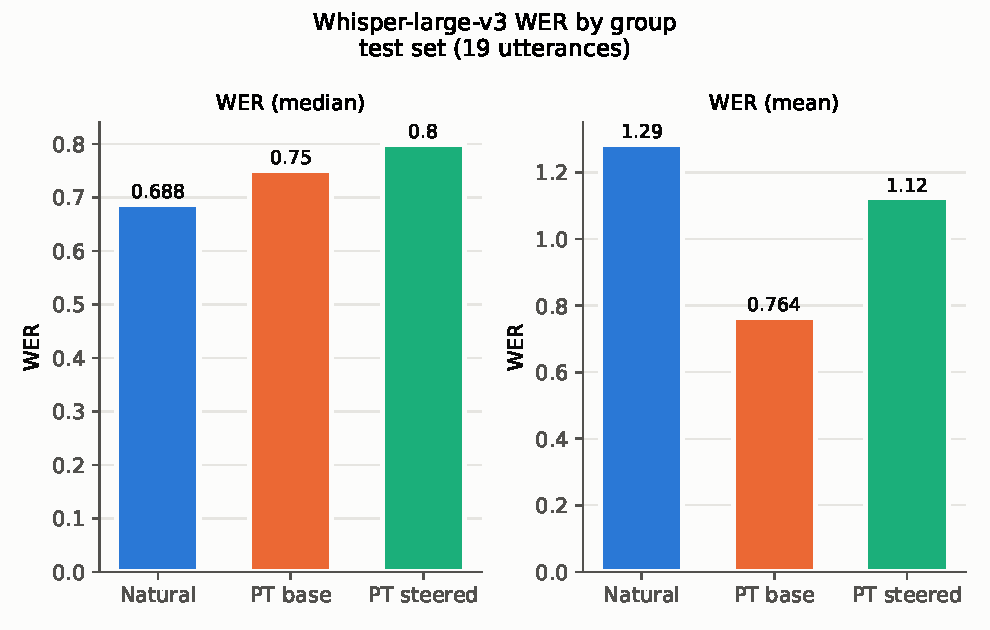
\includegraphics[width=0.8\textwidth]{01_wer_test19.pdf}\caption{WER (Whisper-large-v3), median and mean. Natural WER is high, so WER is a weak intelligibility proxy here.}\end{figure}
\begin{figure}[H]\centering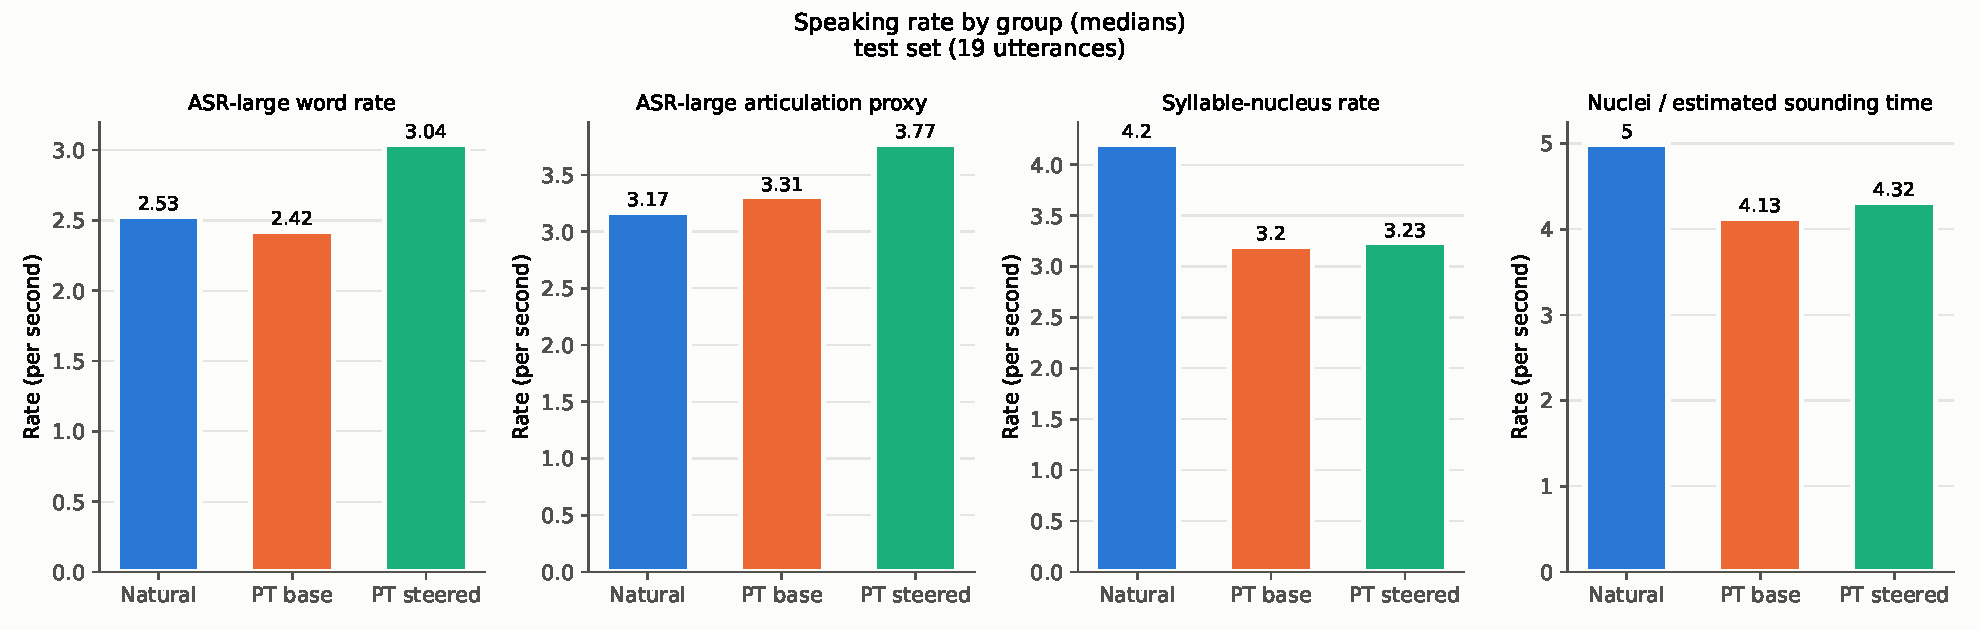
\includegraphics[width=\textwidth]{02_speaking_rate_test19.pdf}\caption{Speaking rate: ASR word rate, articulation proxy, syllable-nucleus rate, nuclei per sounding time.}\end{figure}
\begin{figure}[H]\centering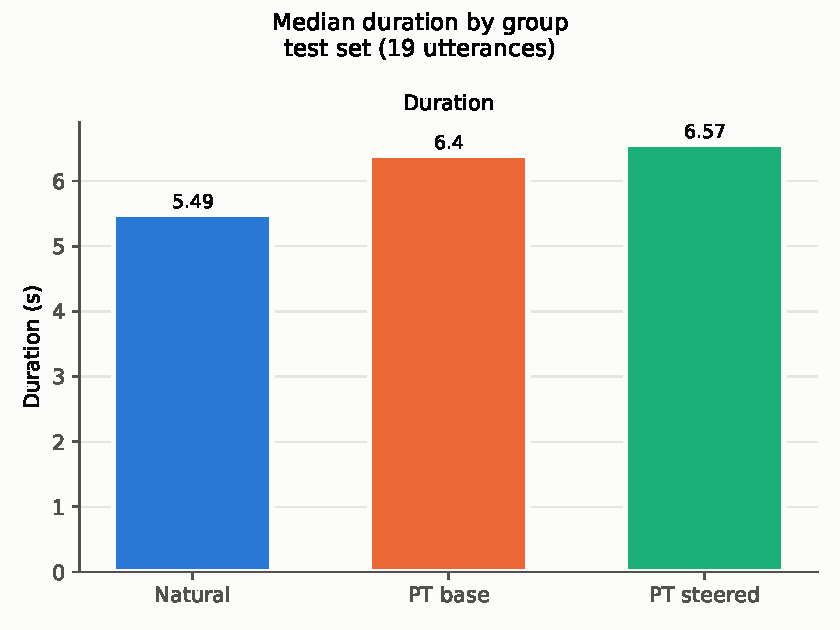
\includegraphics[width=0.55\textwidth]{03_duration_test19.pdf}\caption{Median clip duration.}\end{figure}
\begin{figure}[H]\centering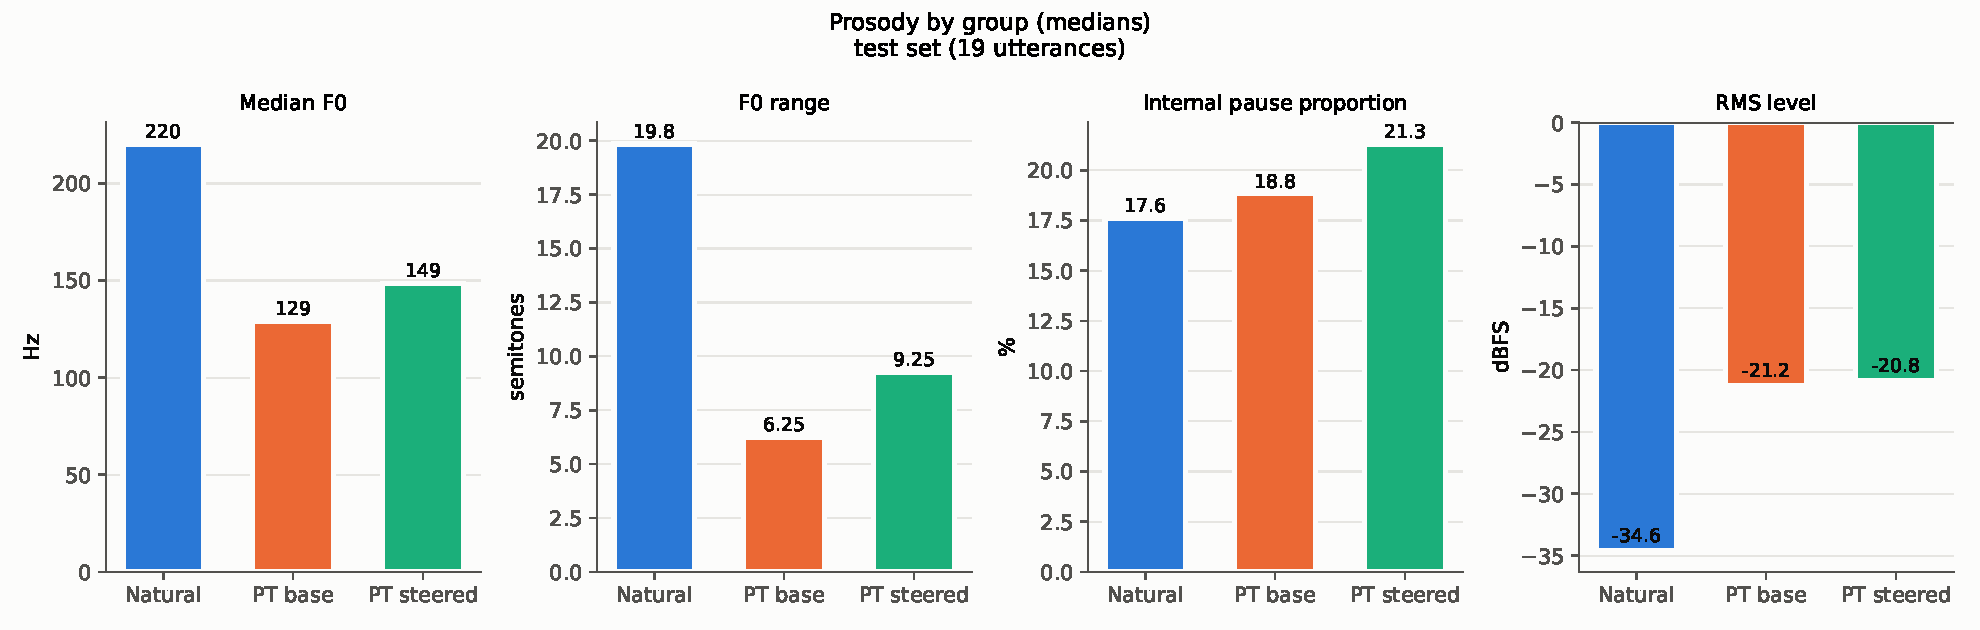
\includegraphics[width=\textwidth]{04_prosody_test19.pdf}\caption{Prosody: median F0, F0 range, internal pause proportion, RMS level.}\end{figure}
\begin{figure}[H]\centering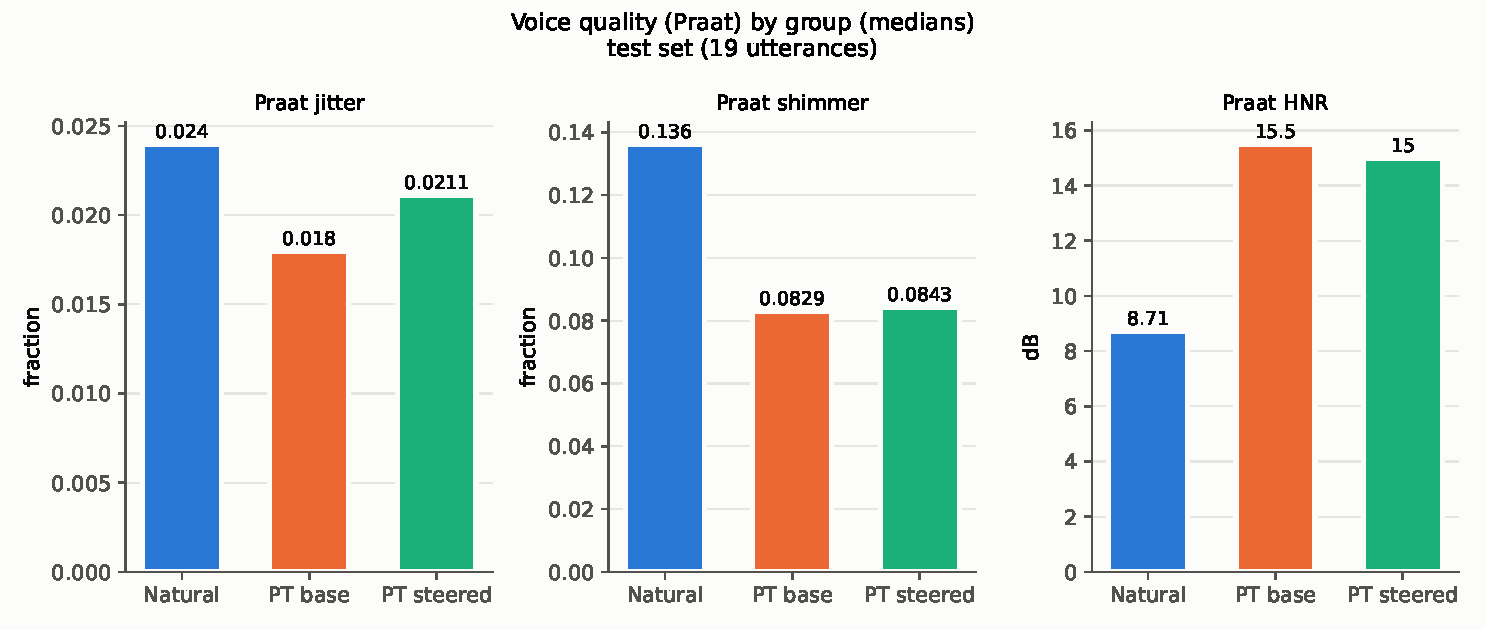
\includegraphics[width=\textwidth]{05_voice_quality_test19.pdf}\caption{Voice quality: jitter, shimmer, HNR.}\end{figure}
\begin{figure}[H]\centering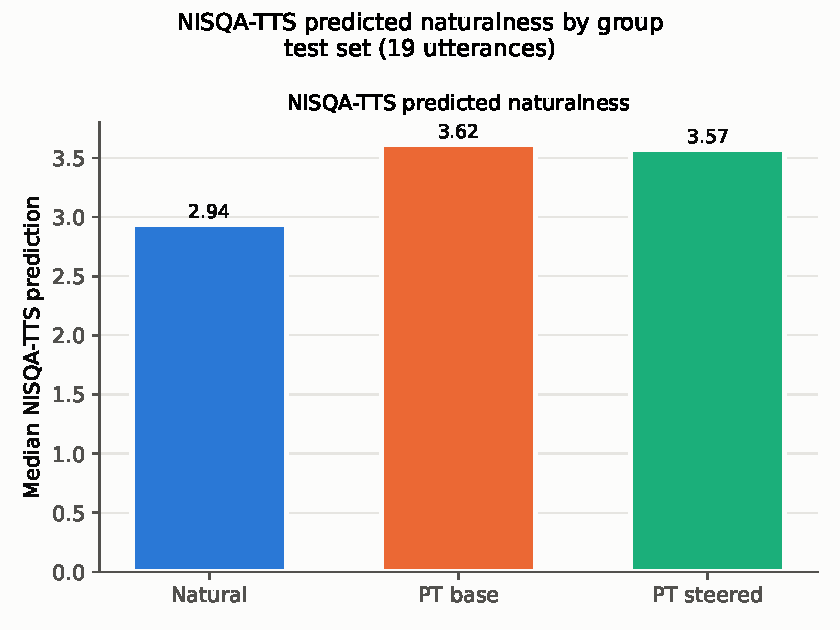
\includegraphics[width=0.55\textwidth]{06_nisqa_test19.pdf}\caption{NISQA-TTS (learned quality score).}\end{figure}
\begin{figure}[H]\centering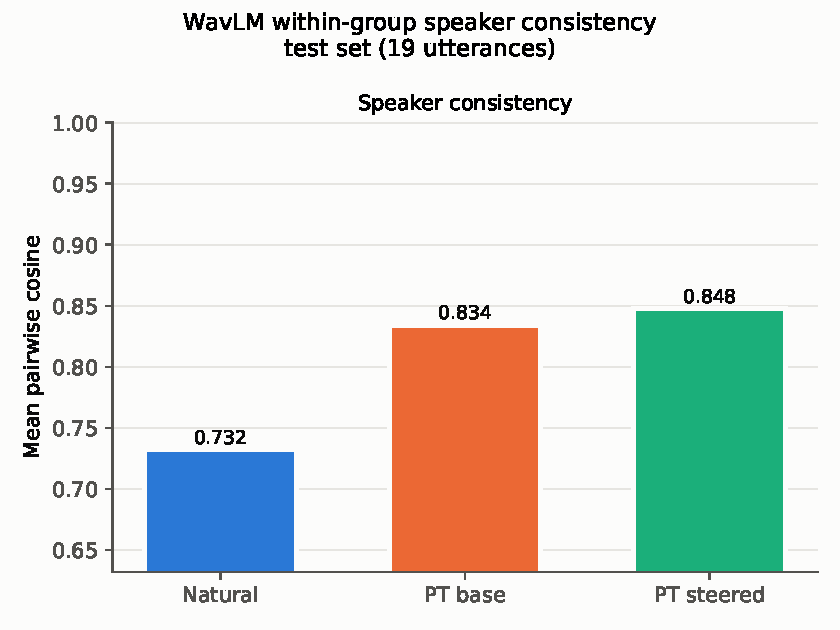
\includegraphics[width=0.55\textwidth]{07_speaker_consistency_test19.pdf}\caption{WavLM within-group speaker consistency (mean pairwise cosine). PT uses a random speaker per clip.}\end{figure}
\begin{figure}[H]\centering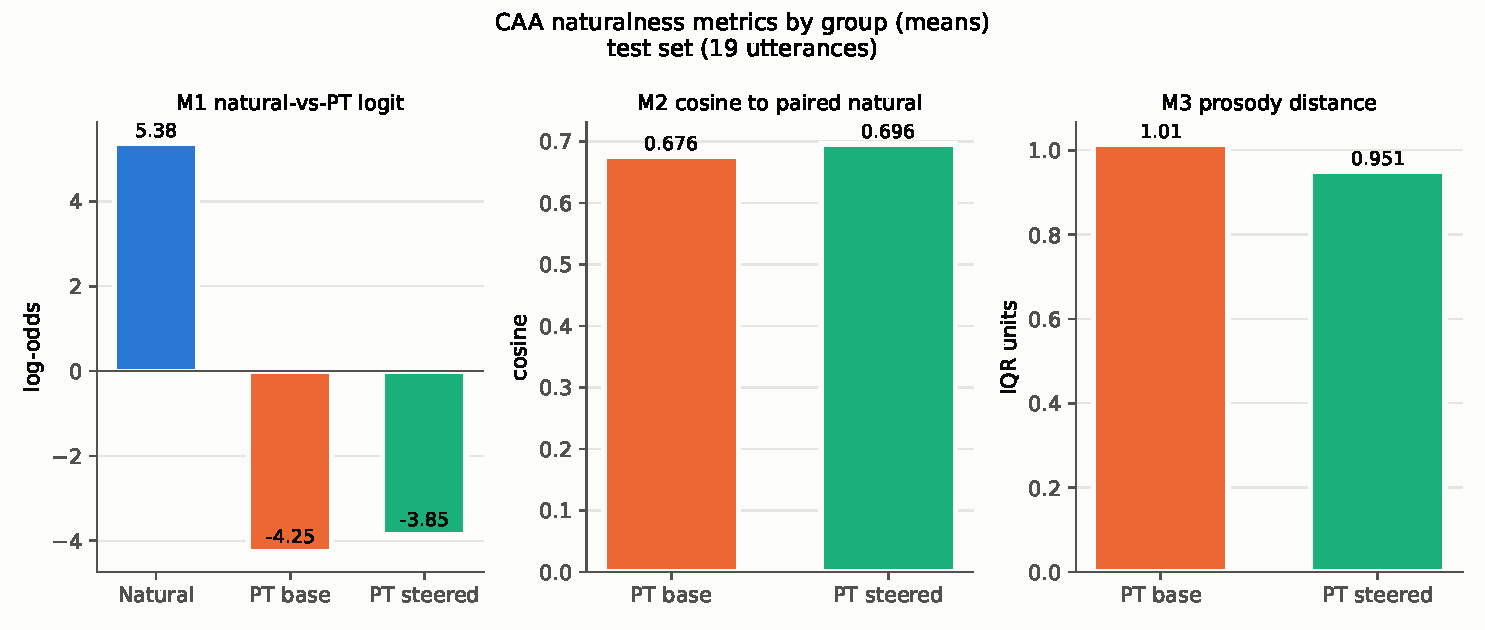
\includegraphics[width=\textwidth]{08_naturalness_m1_m3_test19.pdf}\caption{CAA metrics: M1 natural-vs-PT classifier logit, M2 cosine to paired natural clip, M3 prosody distance (lower is better).}\end{figure}

\section{All 100 utterances (in-sample)}
The steering vector and the M1 classifier used the train utterances, so these numbers are biased in favour of steering.
\begin{figure}[H]\centering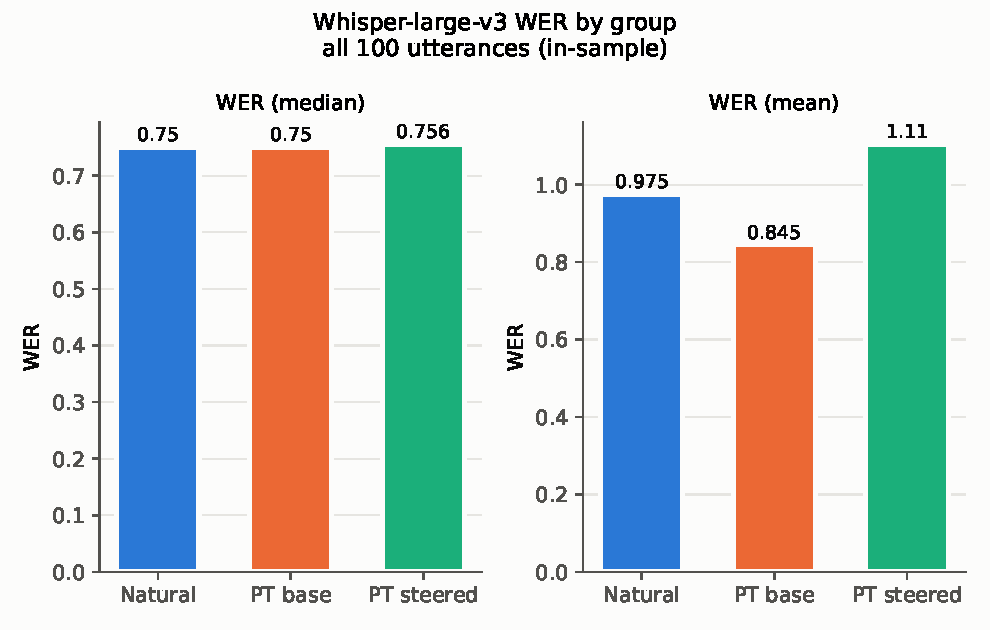
\includegraphics[width=0.8\textwidth]{01_wer_all100_insample.pdf}\caption{WER.}\end{figure}
\begin{figure}[H]\centering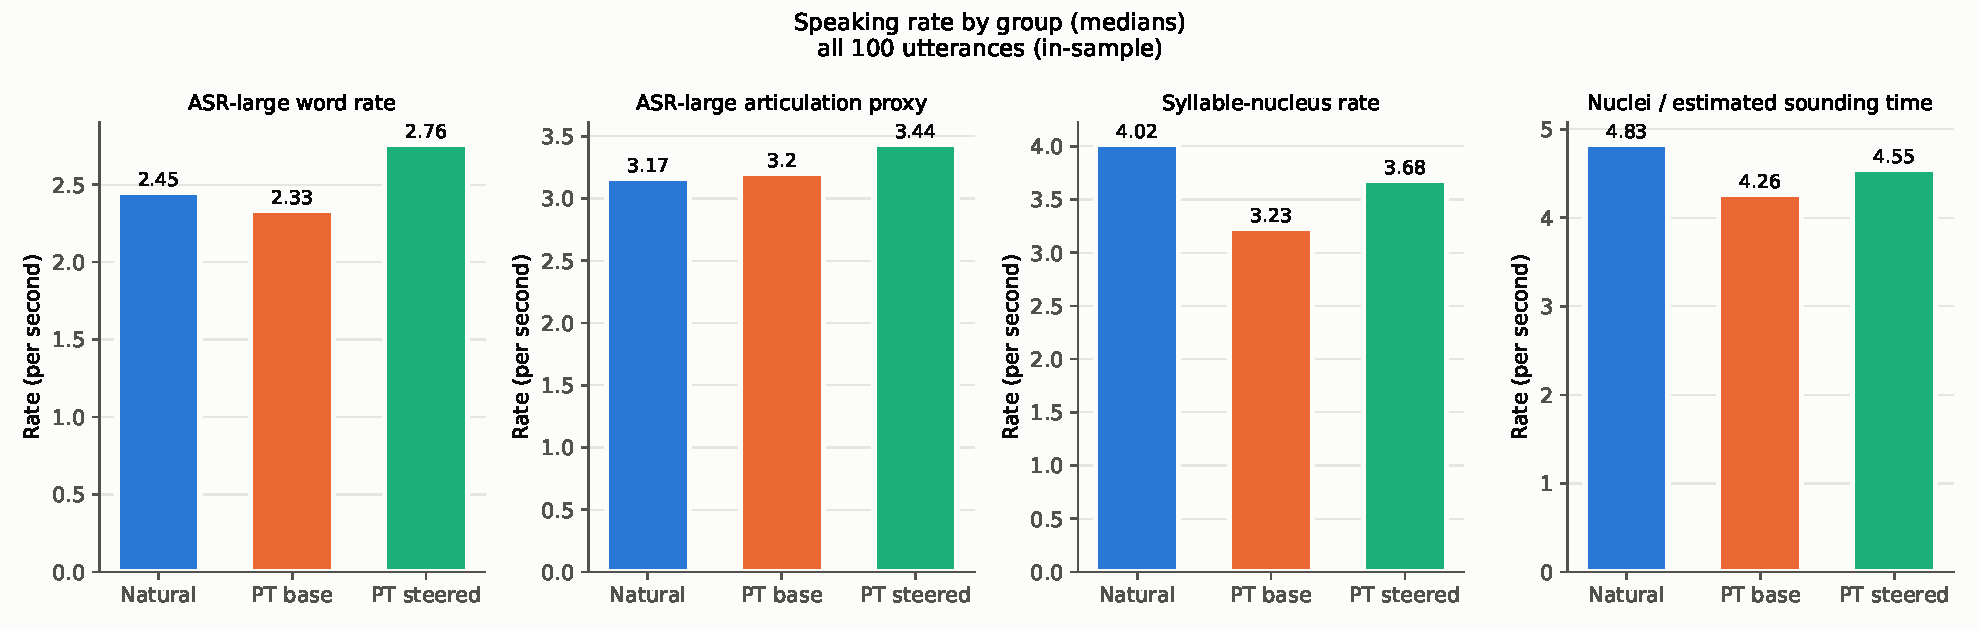
\includegraphics[width=\textwidth]{02_speaking_rate_all100_insample.pdf}\caption{Speaking rate.}\end{figure}
\begin{figure}[H]\centering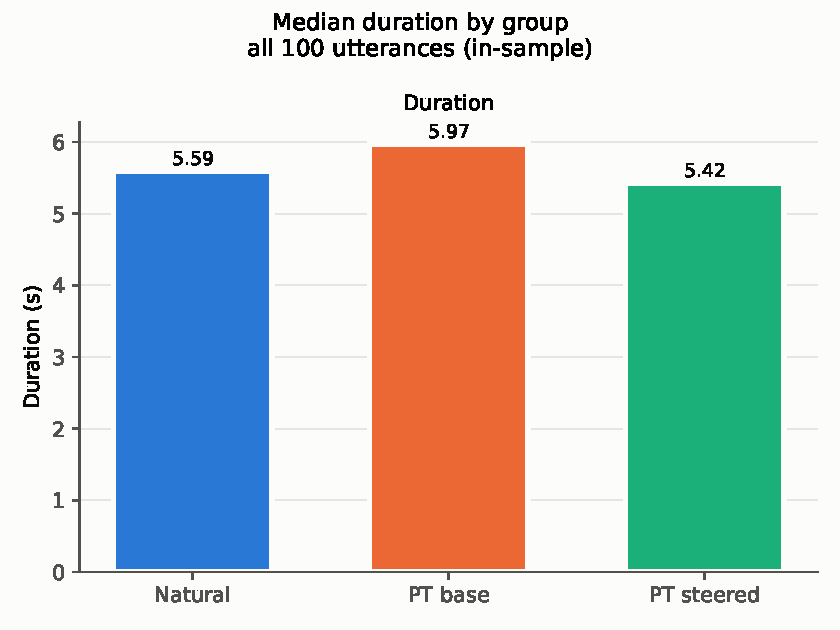
\includegraphics[width=0.55\textwidth]{03_duration_all100_insample.pdf}\caption{Median duration.}\end{figure}
\begin{figure}[H]\centering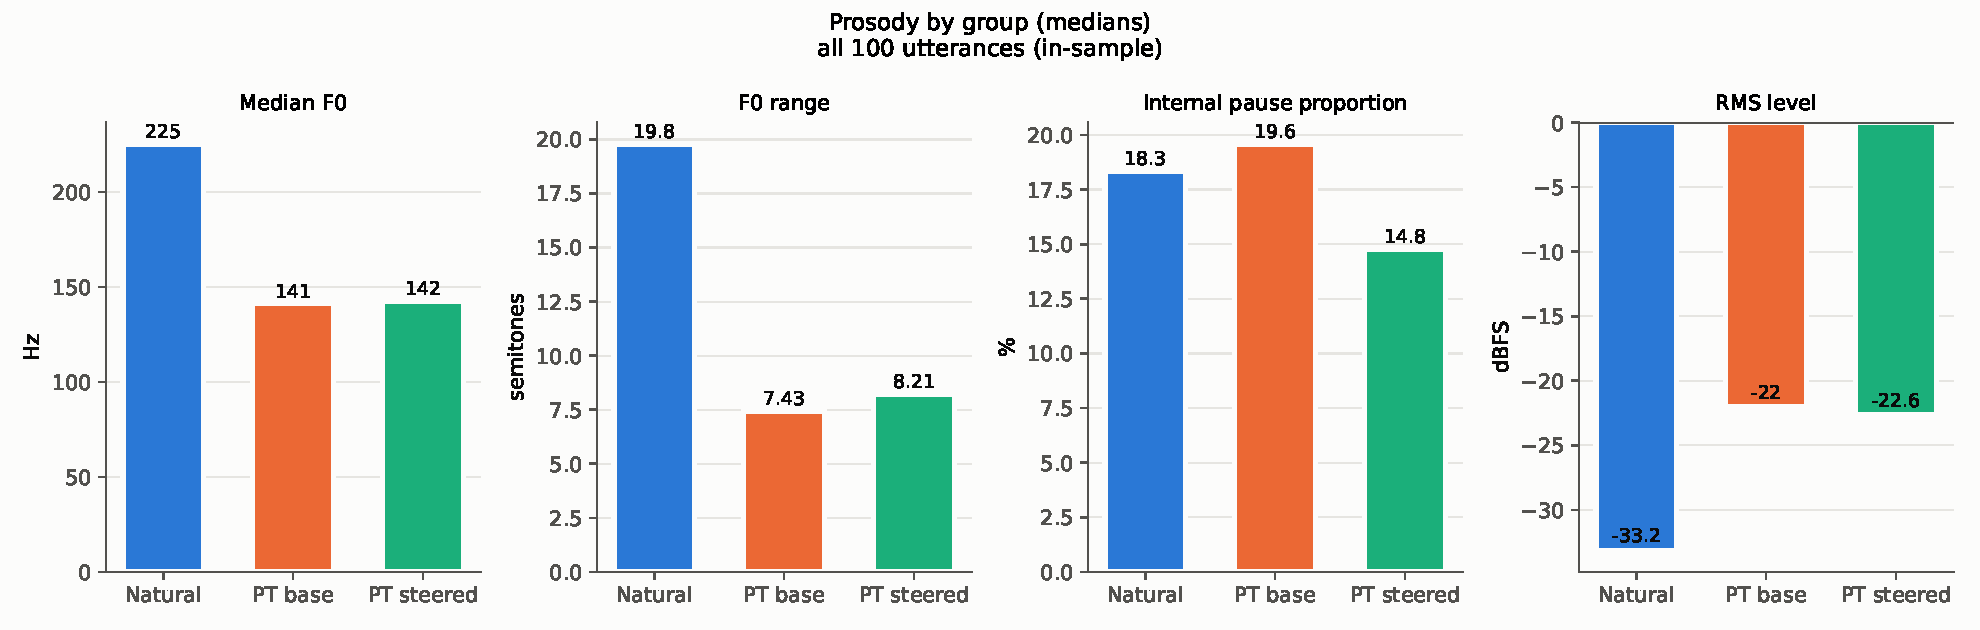
\includegraphics[width=\textwidth]{04_prosody_all100_insample.pdf}\caption{Prosody.}\end{figure}
\begin{figure}[H]\centering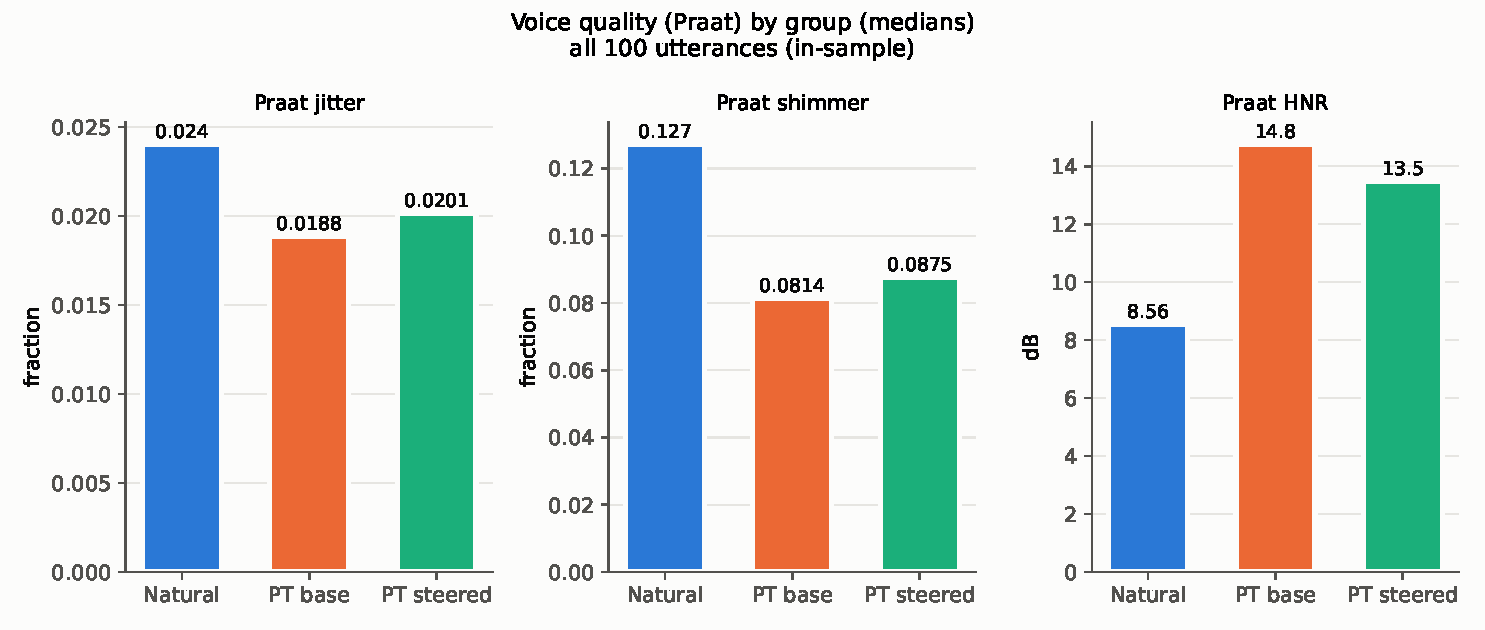
\includegraphics[width=\textwidth]{05_voice_quality_all100_insample.pdf}\caption{Voice quality.}\end{figure}
\begin{figure}[H]\centering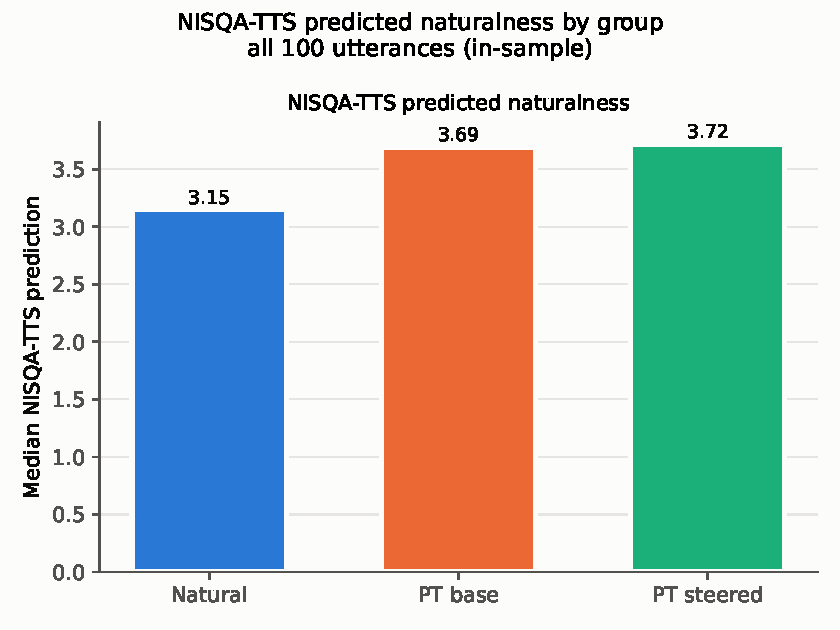
\includegraphics[width=0.55\textwidth]{06_nisqa_all100_insample.pdf}\caption{NISQA-TTS (one steered clip under 0.3\,s unscored).}\end{figure}
\begin{figure}[H]\centering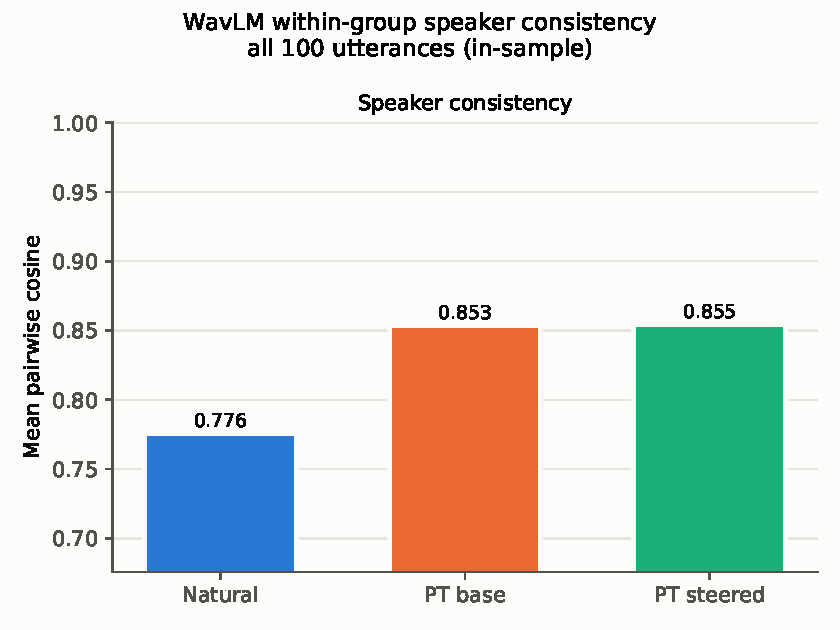
\includegraphics[width=0.55\textwidth]{07_speaker_consistency_all100_insample.pdf}\caption{Speaker consistency.}\end{figure}
\begin{figure}[H]\centering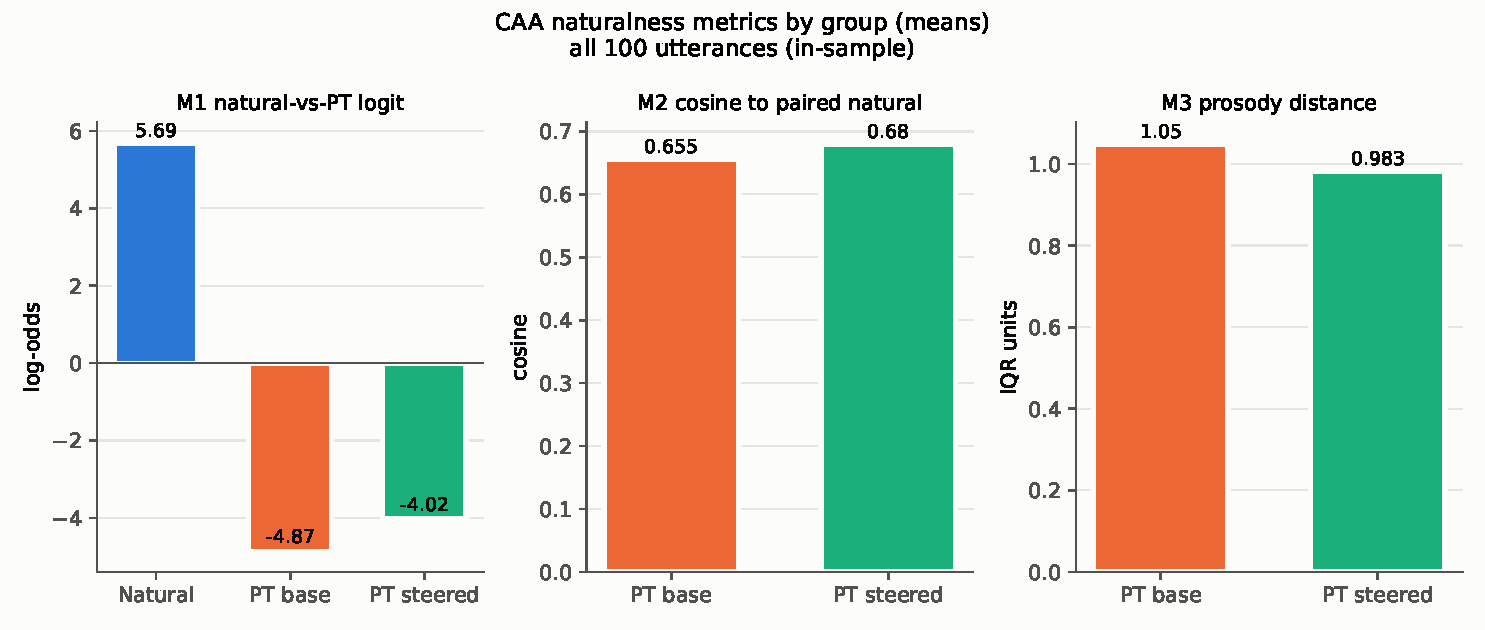
\includegraphics[width=\textwidth]{08_naturalness_m1_m3_all100_insample.pdf}\caption{M1--M3.}\end{figure}

\paragraph{Listening.} \path{/local/speech/users/sp4050/Listening_Examples_100_PT/} on kedi: per utterance, the natural clip, \texttt{TRANSCRIPT.txt}, \texttt{02\_OrpheusPT\_base.wav}, \texttt{03\_OrpheusPT\_steered.wav}; open \texttt{listen.html}.
\end{document}
